\section{Additional Analysis}

The results presented in the last section raised two
additional questions.
In comparison to edit longevity, the performance of ${\approx}29.26\%$
PR-AUC by text longevity is quite poor;
why does text longevity not do so well as edit longevity?
Our second question is about the triangle inequality:
how important is it that our edit distance function satisfy
this property to be a good predictor of vandalism?

\subsection{Edit Longevity Outperforms Text Longevity}

As part of our investigation, we started looking at specific
instances of text longevity values.
In Figure~\ref{fig:ts-GWB-SCBB},
we see the text survival for two different contributions;
both do seem to have the general ``exponential'' shape
that we previously described.
Also computed in each figure is the text longevity measure based on
the 20~revisions shown in each graph, but notice that the text
longevity computed for
Figure~\ref{fig:ts-GeorgeWBush} doesn't exhibit the curve we expect.
Instead of following the text survival, the curve goes below the
level of text which survives each revision.

\begin{figure}[tbph]
\centering
\subfloat
  [article \underline{George W.~Bush}]
  [The text survival graph for the text contributed early
    in the history of article \underline{George W.~Bush}.]
  {
    \framebox{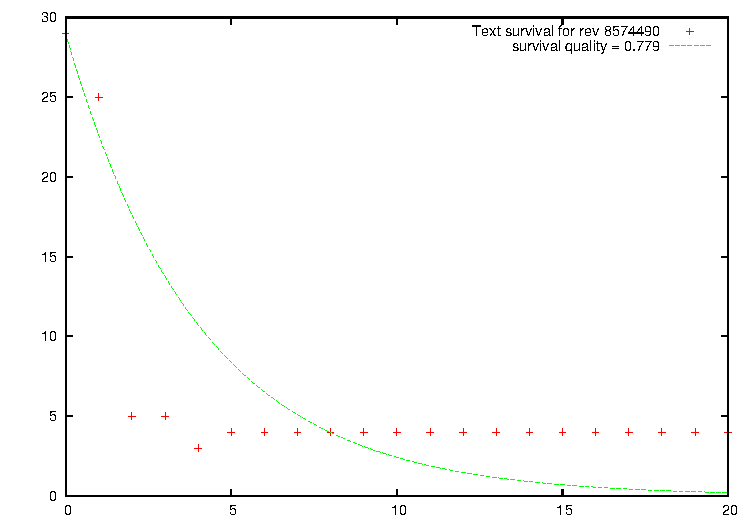
\includegraphics[width=0.45\textwidth]{part-F70-editquality/graph-TS-GeorgeWBush-8574490}}
    \label{fig:ts-GeorgeWBush}
  }
\hspace{1ex}
\subfloat
  [article \underline{Santa Cruz Beach Boardwalk}]
  [The text survival graph for the text initially contributed
	as part of the article \underline{Santa Cruz Beach Boardwalk}.]
  {
    \framebox{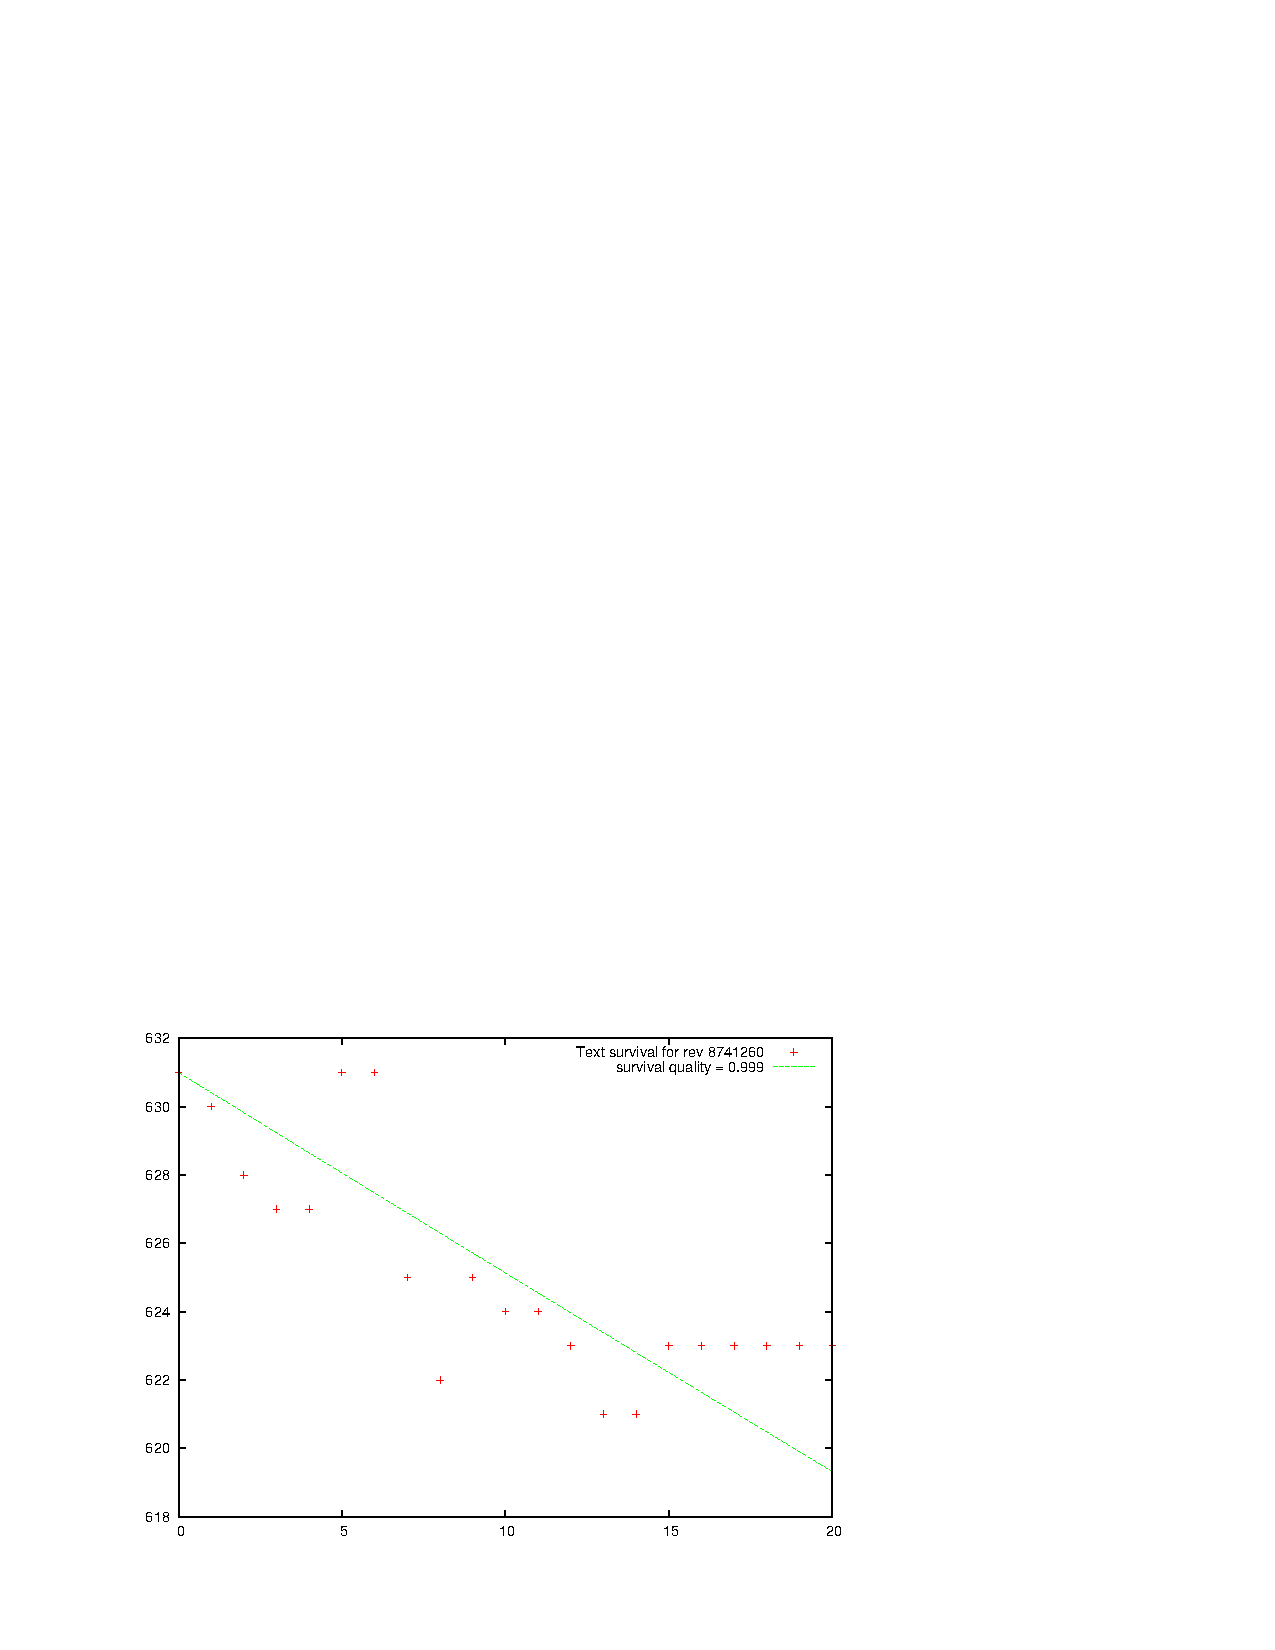
\includegraphics[width=0.45\textwidth]{part-F70-editquality/graph-TS-SantaCruzBeachBoardwalk}}
    \label{fig:ts-SantaCruzBeachBoardwalk}
  }
\caption[The text survival quality graphs for two articles]{
  The text survival quality of two different articles, computed
  based on 20~revisions.
  The majority of the editing happens in the
  revisions immediately after the initial edit, in these two cases.
  \label{fig:ts-GWB-SCBB}
}
\end{figure}

The explanation for this discrepancy turns out to be a flaw in our
thinking about the original model.
While the text survival for contributions does seem to have an
exponential look to it, exponentials do not approach some fixed
non-zero value --- they approach zero.
In order to fit the curve to closely follow the points of text survival,
the last value
(in the case of the data shown in Figure~\ref{fig:ts-GeorgeWBush},
the amount of text that survives after the $20^{th}$ revision)
should be taken as the ``zero reference point'' which is subtracted
from all the values.
Applying our exponential curve fitting technique to these new values
will give a much better approximation to the data.
The problem with this better fit is that it changes the meaning of
a score of zero; instead of meaning that the text was immediately deleted,
a score of zero would mean that the text immediately reached its
final survival level.
In other words, we would be measuring how quickly the text stabilizes,
rather than how much agreement there was that the text belonged in
the article.


\subsection{The Triangle Inequality}
\label{sec:triangle-inequality}

The intuition behind our formulation of edit longevity relies on
the metaphor analogizing the \intro{distance} between two revisions
with the \intro{work} or \intro{effort} that an author puts
into making the edit from one revision to the other;
in particular, it is the triangle inequality (one of the
metric properties of distance) that allows us to say that we
can compute how much effort was \textit{useful} in bringing
the article closer to how it appears in a future revision.

We have explored the use of several different definitions of
the \intro{edit distance} to represent this effort, but
noted that the triangle inequality did not completely hold;
see~\cite{Sankoff1999} for a summary of known conditions under which
the triangle inequality holds for
\intro{listing}, \intro{alignment}, or \intro{trace} distances.

\begin{figure}[htbp]
\centering
  \subfloat[
    listing distance][
    Listing distance is computed by finding the shortest edit script.
    ]{
    \framebox{
      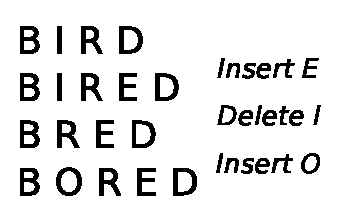
\includegraphics[width=0.4\textwidth]{part-F70-editquality/fig-DiffListing}
    }
  }
  \hspace{2ex}
  \subfloat[
    trace distance
    ][
    Simple trace distance is computed by establishing a correspondence
    between the source and target strings, such that trace lines
    do not cross.
    ]{
    \framebox{
      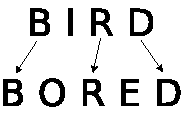
\includegraphics[width=0.4\textwidth]{part-F70-editquality/fig-DiffTrace}
    }
  }
  \\
  \subfloat[
    alignment distance
    ][
    Alignment distance is computed by finding an alignment which
    results in the minimum number of insertions and deletions.
    ]{
    \framebox{
      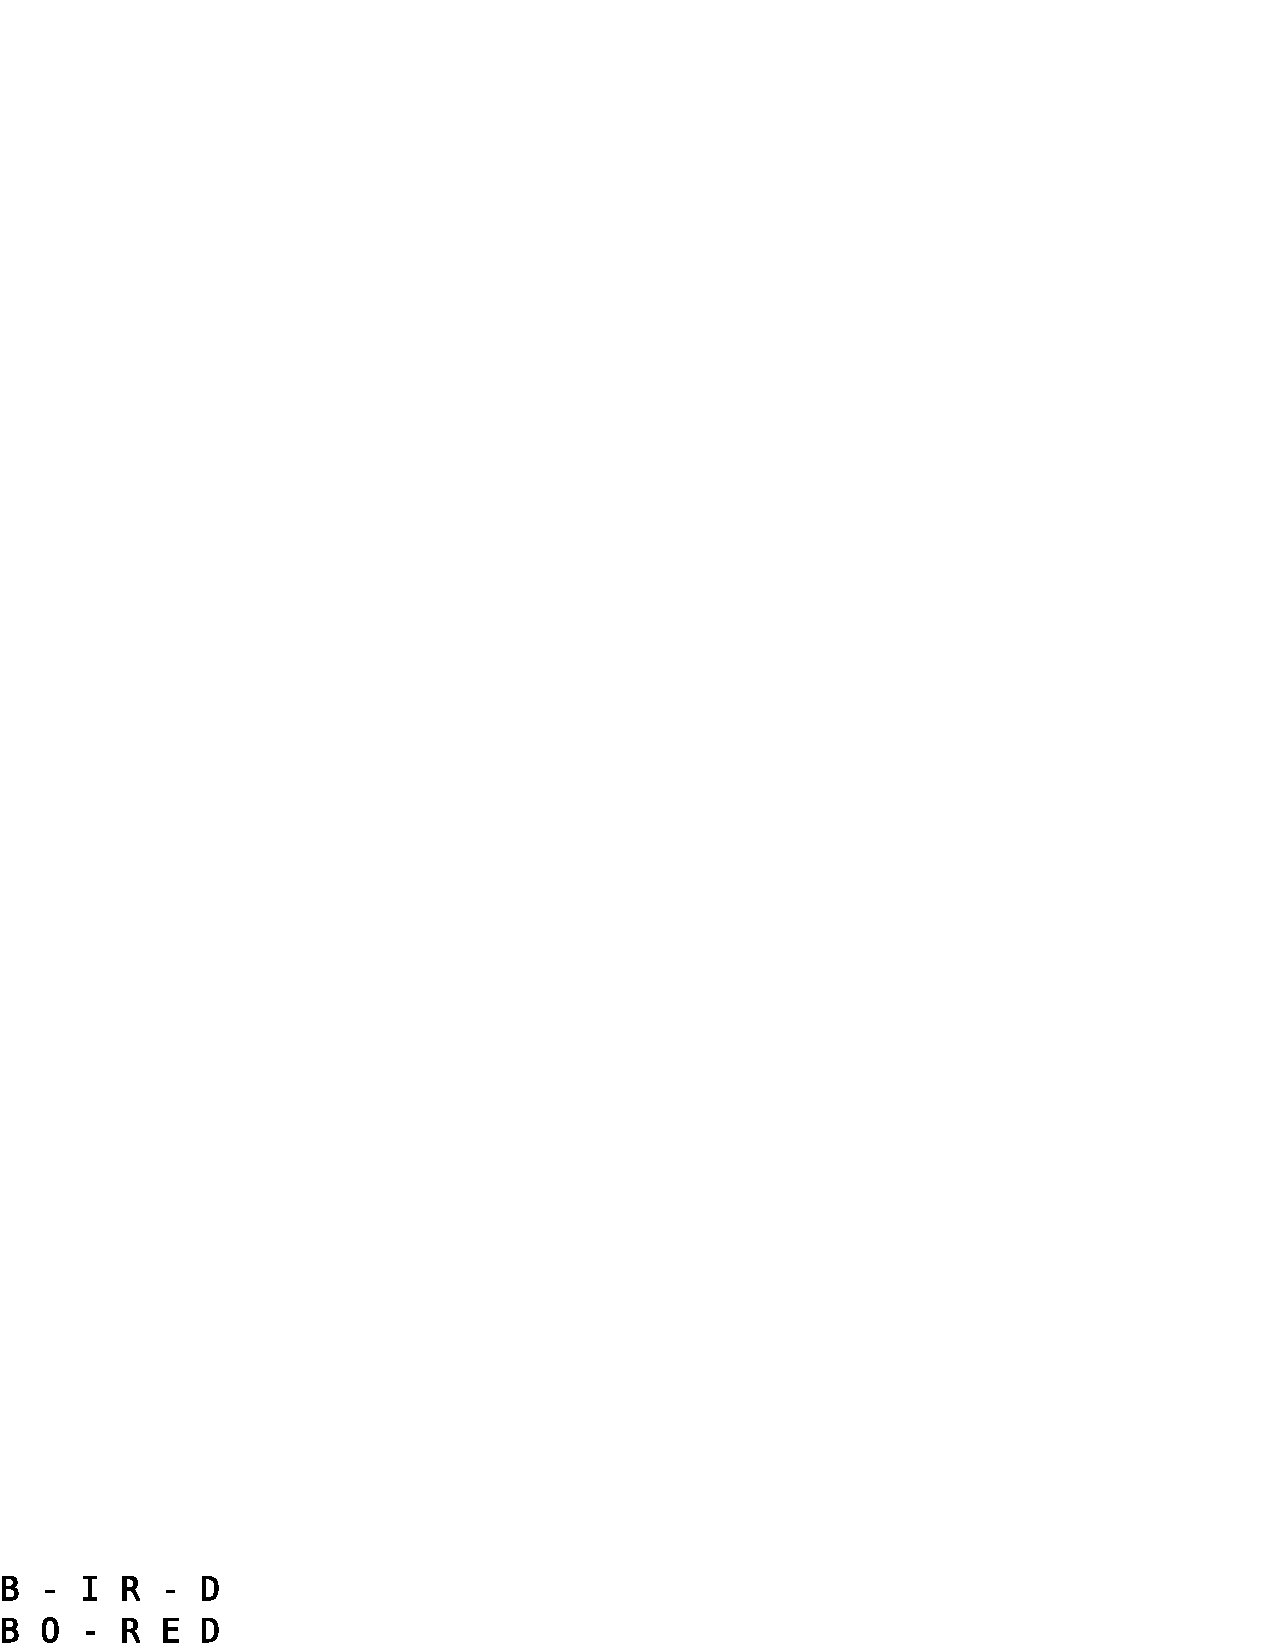
\includegraphics[width=0.4\textwidth]{part-F70-editquality/fig-DiffAlignment}
    }
  }
\caption[Examples of three different styles for computing edit distance]{
  Examples of the three different methods typically used to compute
  edit distance.  See~\cite{Sankoff1999} for an in-depth discussion
  on the distinctions between these methods.
  \label{fig:trace-alignment-listing}
}
\end{figure}

Our particular difference algorithm makes use of
Tichy's block moves~\cite{Tichy1984}, which amounts to computing
the trace that matches the source string to the target string.
That matches are allowed between any parts of the two strings
is equivalent to allowing transpositions as well as the usual
insert and delete operations; the difference we compute does not support
substitutions of one word with another.
There is previous research on allowing
transpositions~\cite{Lowrance1975,Wagner1975,Sankoff1999} in
computing edit distance; our work primarily differs from this
earlier work in that we prefer to select longest matches rather
than minimizing the total edit distance computed.

The various proposals for edit distance that we investigated are
computations derived from the edit script we compute.
Tichy's original counter-example shows that globally greedy algorithms
such as ours do not compute the minimum edit script
(see Figure~\ref{fig:match-comparison}), making it unlikely that
proposed edit distance formulas guarantee the triangle inequality.

\begin{figure}[htbp]
\centering
  \subfloat[
    WikiTrust uses the globally longest match][
    The matching obtained using the WikiTrust method of
      determining all matches and selecting the longest matches first.
    ]{
    \framebox{
      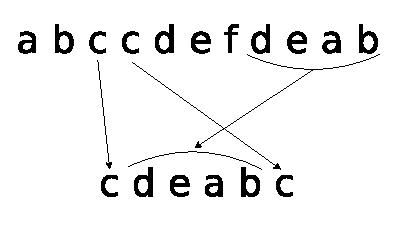
\includegraphics[width=0.4\textwidth]{part-F70-editquality/fig-MatchingGlobal}
    }
  }
  \hspace{2ex}
  \subfloat[
    Tichy uses best match from left-to-right
    ][
    The matching obtained using the Tichy method of scanning
      the target string from left-to-right and selecting
      the longest match found in the source string.
    ]{
    \framebox{
      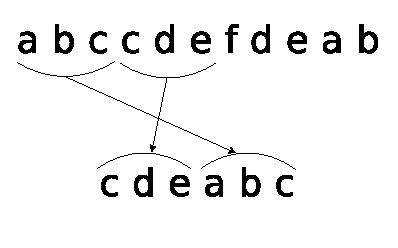
\includegraphics[width=0.4\textwidth]{part-F70-editquality/fig-MatchingLocal}
    }
  }
\caption[An example of when WikiTrust and Tichy differ in matching.]{
  An example of how the matching between a source string and target string
  can differ between WikiTrust's greedy preference for the longest match
  anywhere between the two strings, and Tichy's processing of the
  target string from left-to-right and selecting the longest match
  for the given starting position in the target string.
  This example is based on Tichy's original example demonstrating that
  a globally greedy algorithm does not result in the minimum number of
  operations~\cite{Tichy1984}.
}
\label{fig:match-comparison}
\end{figure}

We present in Appendix~\ref{app:editlong-data} data on the frequency
with which the triangle inequality holds for the various combinations
of difference algorithms and edit distance formulae; only formula~\textbf{ed2}
never violates the triangle inequality.
This is relatively easy to see by an enumeration of the cases, but it
is instructive to examine~\textbf{ed1} first.

To show that~\textbf{ed1} does not satisfy the triangle inequality, we
note that the definition
    \begin{equation*}
    I_{tot} + D_{tot}
    \end{equation*}
is amenable to the \intro{weighted operation} notation used
throughout~\cite{Sankoff1999}.
In this notation, an insertion of word $x$ is said to
contribute weight $w(\phi, x)$ to the final edit distance, and
deletion of word $x$ contributes weight $w(x, \phi)$.
We extend the notation to represent the contribution of a
Move operation on $x$ as $w(x, x)$.
Edit distance~\textbf{ed1} can then be described as the following
assignment of weights:
\begin{align*}
  w(\phi, x) &= 1 \\
  w(x, \phi) &= 1 \\
  w(x, x) &= 0
\end{align*}
For convenience, we represent the situation where a word is in
neither the source nor target revision as $w(\phi, \phi)$ and
assign it a weight of zero.
Note that~\textbf{ed1} assigns a weight of zero to Move operations,
so we do not need to concern ourselves with the location of word~$x$
in the source and target strings.

We consider three revisions, just as we did in analyzing
edit longevity in Figure~\ref{fig-editcontr}: \version{k-1},
\version{k}, and \version{j}.
To verify the triangle inequality,
\begin{equation*}
  \dist{}{k-1,k} + \dist{}{k,j} \ge \dist{}{k-1,j},
\end{equation*}
we enumerate the possible cases of word $x$ existing in each
revision:
\begin{enumerate}
\item word $x$ exists in revision \version{k-1}, but not in
  \version{k} nor \version{j}.
  This translates into deletion operations for \dist{}{k-1,k}
  and \dist{}{k-1,j}, so that we have
  \begin{align*}
    w(x, \phi) + w(\phi, \phi) \ge w(x, \phi),
  \end{align*}
  which is true.
\item word $x$ exists in revision \version{k}, but not in
  \version{k-1} nor \version{j}.
  \begin{align*}
    w(\phi, x) + w(x, \phi) & \ge w(\phi, \phi).
  \end{align*}
\item word $x$ exists in revision \version{j}, but not in
  \version{k-1} nor \version{k}.
  \begin{align*}
    w(\phi, \phi) + w(\phi, x) & \ge w(\phi, x).
  \end{align*}
\item word $x$ exists in revision \version{k-1} and \version{k}, but not in
  \version{j}.
  \begin{align*}
    w(x, x) + w(x, \phi) & \ge w(x, \phi).
  \end{align*}
\item word $x$ exists in revision \version{k-1} and \version{j}, but not in
  \version{k}.
  \begin{align*}
    w(x, \phi) + w(\phi, x) & \ge w(x, x).
  \end{align*}
\item word $x$ exists in revision \version{k} and \version{j}, but not in
  \version{k-1}.
  \begin{align*}
    w(\phi, x) + w(x, x) & \ge w(\phi, x).
  \end{align*}
\item word $x$ exists in all of revisions \version{k-1}, \version{k},
  and \version{j}.
  \begin{align*}
    w(x, x) + w(x, x) & \ge w(x, x).
  \end{align*}
\end{enumerate}

All of these statements are true, so it would seem that
edit distance~\textbf{ed1} satisfies the triangle inequality.
The complication arises in the requirement
that there be a minimum number of words to be considered a
Move operation.
This restriction means that it is possible for a word to exist
in both revisions, but be considered a Deletion and Insertion.
For example, if word $x$ exists in all three revisions, a different
possible analysis is:
  \begin{align*}
    w(x, x) + w(x, x) & \ge w(x, \phi) + w(\phi, x),
  \end{align*}
which does not hold true, and thus the triangle inequality sometimes
will break down.

\bigskip

The proof that edit distance~\textbf{ed2} always satisfies the
triangle inequality follows a similar analysis, but using different
weights:
\begin{align*}
  w(\phi, \phi) &= 0 \\
  w(\phi, x) &= 1 \\
  w(x, \phi) &= 1 \\
  w(x, x) &= 1
\end{align*}
These weights result in every statement holding true, even the
alternative analysis, so that the
full triangle inequality also holds true.

Examining the performance of \textbf{ed2} in
Appendix~\ref{app:editlong-data}, we note that it was far from the best
performing definition of edit distance in terms of predicting vandalism
in the PAN-WVC-10 dataset.
Although using an edit distance formulation that satisfies the triangle
inequality is desirable, it is not sufficient to achieve good
performance.
The goal of an edit distance function in our context is to estimate
the amount of \intro{effort} that an author expends in creating an
edit from one revision to another.
We chose to follow a model which prefers the longest possible match
between source and target revisions, but another viable route is to
minimize the amount of text which is rearranged (\ie minimize the
number of transpositions)~\cite{Wagner1975}.
We leave as an open question how to best characterize the work
that an author does.

